\subsection{Mismatched Crowdsourcing}
\label{sec:MC}

As described in \ref{sec:bgmc}, mismatched crowdsourcing gives crowd
workers speech in an unfamiliar language, which they treat as a sequence
of nonsense syllables and transcribe using their native-language 
orthography (Fig.~\ref{fig:mc}).

\begin{figure}
  \centerline{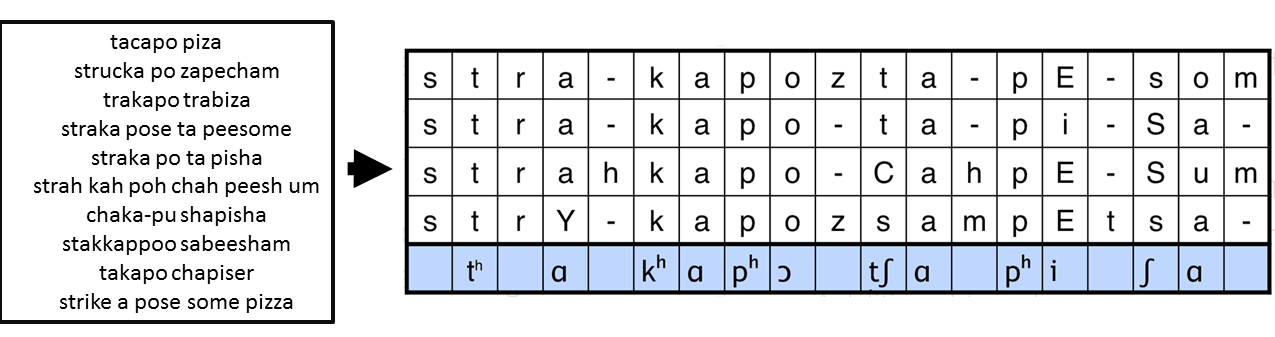
\includegraphics[width=5in]{../figs/fig_jyothi.png}}
  \caption{In mismatched crowdsourcing, people who don't speak a
    language (in this case Swahili) are asked to transcribe it using
    nonsense syllables in the orthography of their own language (in
    this case English).  There is a great deal of variability in their
    responses (left), but information about the phonetic content of
    the speech can be derived by merging the transcripts (top four
    rows at right) and decoding using a model of non-native speech
    perception (decoding result in the bottom row at right).}
  \label{fig:mc}
\end{figure}
%% comments: it's odd that all four of the illustrated transcripts begin
%% with the sequence [str], but the decoded result does not include the
%% [s] or the [r]. Perhaps it would be better to choose four transcripts
%% that vary more widely (and even indicate which orthographic strings
%% they correspond to) so that the derived result looks more plausible.
%% It is also odd that the formation of lambda involves choosing 5 best
%% MTs, but the figure shows 4 MTs.
%% Also, it is odd that pseudo-phonetic code is used in the transcripts
%% instead of IPA; IPA only occurs in the decoded result. Is there a
%% compelling reason for that?  Also, this figure is an excellent
%% candidate for vector graphic format rather than raster, since it's
%% all lines and text. I'm happy to help out with recreating figures in
%% vector format if that's desired.
%% Finally, I think this figure belongs after the following paragraph,
%% which could sensibly be merged into the opening paragraph of this
%% section. 

Given a set of mismatched transcripts $T$, we can compute a distribution 
over phone sequences $\phi$ in the utterance language (referred to as
probabilistic transcripts or PTs).  
As an intermediate step towards this goal, prior
work~\cite{JHJ15b} developed techniques to merge the transcripts
in $T$ into a distribution $\Pr(\lambda|T)$ over ``representative
transcripts'' in the orthography of the annotation language, denoted
by $\lambda$. Formation of $\lambda$ from $T$ involves data filtering
(choosing the most representative 5 transcripts out of each set of 10,
using pair-wise string edit distances among the transcripts),
conversion of annotation-language orthography into a pseudo-phonetic
code in order to represent common letter sequences (e.g., ``ee'' in
English orthography represents the phoneme \ipa{/i/}), and a weighted
voting scheme in which the weight of each transcript is proportional
to the frequency with which it matches the other transcripts.

%% Unclear point (maybe just to me): What exactly is lambda? In the
%% previous paragraph it's described as the set of representative
%% transcriptions, whereas in the next paragraph it is described as a
%% confusion network, and in a later paragraph seems to be used to refer
%% to (the set of) "graphemes in the annotation language".
Once transcripts in the orthography of the transcriber language have been
aligned and filtered to create the confusion network $\lambda$, they
are then translated into a distribution over phonemic transcriptions
(Fig.~\ref{fig:mc}, shaded boxes) according to:
\begin{align}
  \rho(\phi|T) &=
  \sum_{\lambda} \rho(\phi, \lambda|T) =
  \sum_{\lambda} \rho(\phi|\lambda,T) \rho(\lambda|T) \notag \\
  &\approx \max_{\lambda}  \rho(\phi|\lambda) \rho(\lambda|T) \notag \\
  &= \max_{\lambda}  \left(\frac{\rho(\lambda|\phi)}{\rho(\lambda)}
  \rho(\phi)\right) \rho(\lambda|T) 
\label{eq:PT}
\end{align}

The terms other than $\rho(\lambda|T)$ in Equation~\ref{eq:PT} are
estimated as follows.  $\rho(\lambda)$ is modeled using a simple
context-free prior over the letter sequences in $\lambda$.
$\rho(\phi)$ is modeled using a bigram phone language model, trained
on a corpus of Wikipedia text in the target language, converted into
phone sequences as described in Section~\ref{sec:phonotactic}.

$\rho(\lambda|\phi)$ is called the misperception G2P, as it maps to
graphemes in the annotation language, $\lambda$, from phonemes in the
utterance language, $\phi$.  This section describes methods that 
estimate $\rho(\lambda|\phi)$ directly; Section~\ref{sec:eegchanmod} 
describes methods that decompose $\rho(\lambda|\phi)$ 
into separate misperception and G2P transducers.
%% shouldn't it be called "misperception P2G" instead of G2P?

The misperception G2P ($\rho(\lambda|\phi)$) can be trained directly 
using the Carmel toolkit
\cite{Carmel} as a probabilistic finite state transducer mapping
phones to letters, based on representative transcripts $\lambda$ (and
their corresponding native transcripts) for speech {\em in languages
other than the target language}. We assume that misperceptions
depend more heavily on the annotation language than on the utterance
language, and that therefore a model $\rho(\lambda|\phi)$ trained
using a universal phone set for $\phi$ is also a good model of
$\rho(\lambda|\phi)$ for the target language. Note that, while this
assumption is not entirely accurate, it is necessitated by the
requirement that no native transcriptions in the target language can
be used in building any part of our system.
%We also allow this FST to delete phones and insert letters.

\begin{table}[t]
\centering
\begin{tabular}{| c || c | c |}
\hline
Language Code & Dev set (1-best) & Eval set (1-best) \\
\hline
arb & 65.8 & 66.2 \\
yue & 66.4 & 67.8 \\
nld & 68.9 & 70.9 \\
hun & 63.7 & 63.5 \\
cmn & 70.9 & 69.6 \\
swh & 47.6 & 50.3 \\
urd & 67.2 & 70.5  \\
\hline
\end{tabular}
\caption{1-best probabilistic phone transcription error rates on the development and evaluation sets.}
\label{tab:LPER}
\end{table}
%% This table is premature, as the particular languages used for
%% training and test have not yet been defined (and should not be, since
%% this section is about the algorithms used, not the actual experiment).
%% Most of the text in the following paragraph should also move to a
%% later section for the same reason.

A crude measure of the quality of the PTs is given by the phone error
rate between $\phi^* = \argmax_{\phi} \rho(\phi|T)$ and the reference
phone sequences. Table~\ref{tab:LPER} lists these 1-best error rates
on the SBS development and evaluation sets, for all seven
languages. However, the 1-best error rates do not accurately reflect
the extent of information in the PTs that can be leveraged during ASR
adaptation. A fuller picture is obtained by considering a collection
of sequences $\phi$ that are almost as probable as $\phi^*$ according
to our model. Figure~\ref{fig:listPER} shows the trend of phone error
rates (for three languages) obtained by using collections $\phi$ of
increasing size, plotted against an entropy estimate of $\phi$. This
estimate measures the average entropy of phones in the sequences in
$\phi$; e.g., 1 bit of entropy allows two equally probable choices for
each phone in $\phi$. We note that the phone error rates significantly
drop across all languages, staying within 1 bit of entropy per phone,
illustrating the extent of information captured by the PTs.

\begin{figure}[t!]
\begin{center}
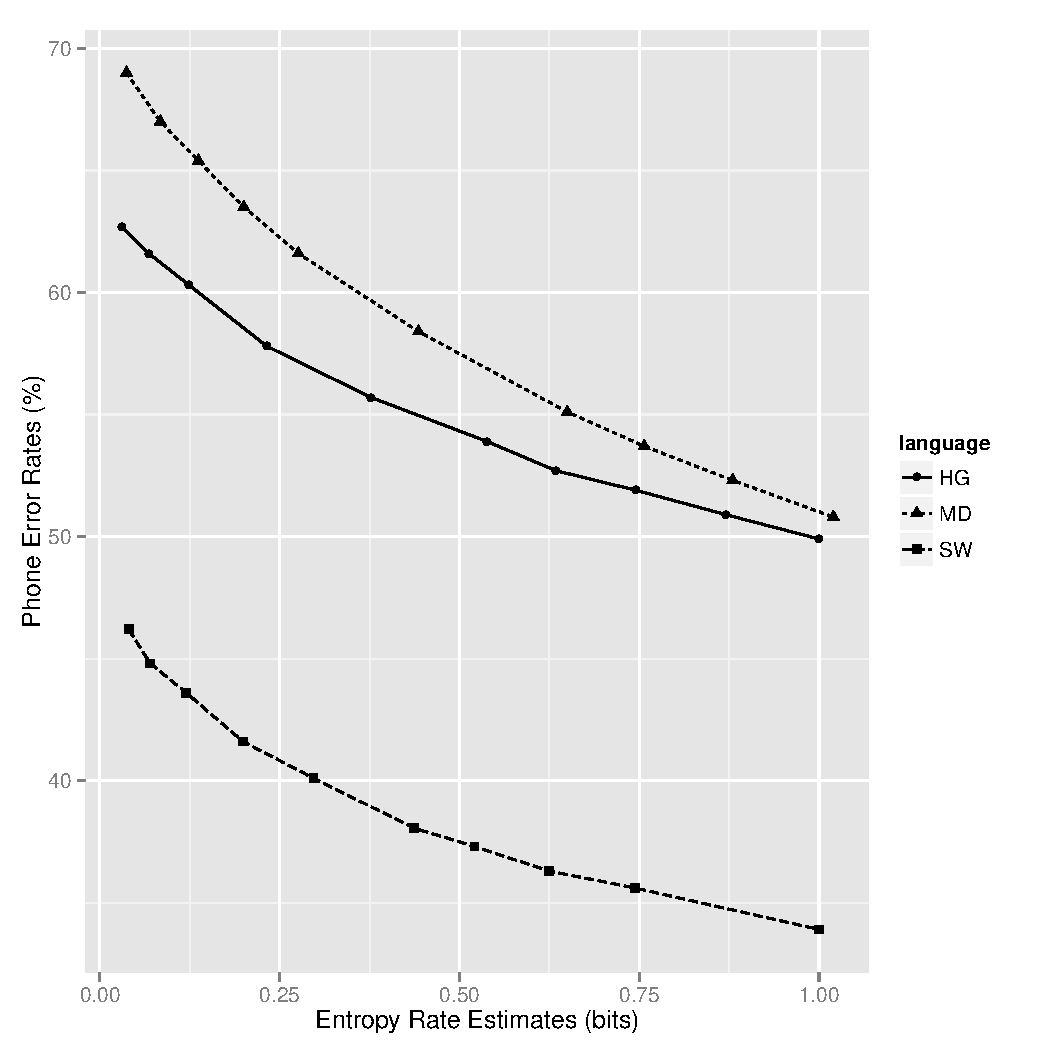
\includegraphics[width=2in]{../figs/listper.pdf}
\end{center}
\caption{Phone error rates plotted against entropy rate estimates of phone sequences in three different languages.}
\label{fig:listPER}
\end{figure}
%% Figure belongs in results section, not here. Annotations are
%% illegible. Note also the language abbreviations issue.
